% -----------------------------------------------------------------------------
% The MIT License (MIT)
%
% Copyright (c) 2015 Pejman Ghorbanzade
%
% Permission is hereby granted, free of charge, to any person obtaining a copy
% of this software and associated documentation files (the "Software"), to deal
% in the Software without restriction, including without limitation the rights
% to use, copy, modify, merge, publish, distribute, sublicense, and/or sell
% copies of the Software, and to permit persons to whom the Software is
% furnished to do so, subject to the following conditions:
%
% The above copyright notice and this permission notice shall be included in
% all copies or substantial portions of the Software.
%
% THE SOFTWARE IS PROVIDED "AS IS", WITHOUT WARRANTY OF ANY KIND, EXPRESS OR
% IMPLIED, INCLUDING BUT NOT LIMITED TO THE WARRANTIES OF MERCHANTABILITY,
% FITNESS FOR A PARTICULAR PURPOSE AND NONINFRINGEMENT. IN NO EVENT SHALL THE
% AUTHORS OR COPYRIGHT HOLDERS BE LIABLE FOR ANY CLAIM, DAMAGES OR OTHER
% LIABILITY, WHETHER IN AN ACTION OF CONTRACT, TORT OR OTHERWISE, ARISING FROM,
% OUT OF OR IN CONNECTION WITH THE SOFTWARE OR THE USE OR OTHER DEALINGS IN
% THE SOFTWARE.
% -----------------------------------------------------------------------------

\section*{Question 1}
An alarm clock is simple to use.
You set the alarm, it rings, you snooze and the last two steps are repeated in a \texttt{while(true)} loop! Write a class \texttt{AlarmClock.java} that defines basic functionalities of an alarm clock: setting an alarm, snoozing and dismissing it.

Use your class in a program \texttt{AlarmClockTest.java} where user is asked to set an alarm.
Every ten seconds your program should check if it's time to ring.
After ringing, user is asked either to snooze or dismiss the alarm.
If snoozed, the alarm is set to ring 5 minutes later.
If dismissed, the alarm is deactivated.

\begin{figure}[H]\centering
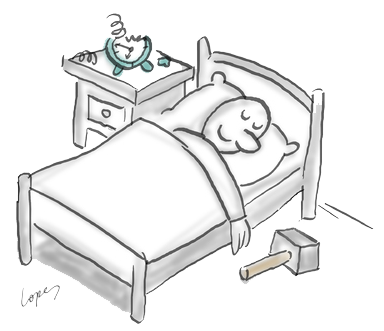
\includegraphics[width=8cm]{\topDirectory/template/images/clock.png}
\end{figure}
\newpage
\subsection*{Solution}
\begin{enumerate}
\item Class \texttt{BankAccount.java}:
\lstset{language=java}
\begin{lstlisting}
public class AlarmClock {
	// 1. Data Members
	private int currentTime;
	private int alarmTime;
	private boolean alarmState;
	// 2. Methods
	public void forwardTime(int seconds) {
		this.currentTime += seconds;
		System.out.println("Current Time is "+ this.getCurrentTime());
	}
	public void reset() {
		this.currentTime = 0;
	}
	public void dismiss() {
		setAlarmState(false);
	}
	public void snoozeAlarm(int snoozeTime) {
		setAlarmTime(currentTime + snoozeTime);
	}
	public boolean isRinging() {
		return (this.alarmTime <= this.currentTime && this.getAlarmState()) ? true : false;
	}
	// 3. Getters and Setters
	public int getCurrentTime() {
		return currentTime;
	}
	public void setCurrentTime(int currentTime) {
		this.currentTime = currentTime;
	}
	public int getAlarmTime() {
		return alarmTime;
	}
	public void setAlarmTime(int alarmTime) {
		this.alarmTime = alarmTime;
	}
	public boolean getAlarmState() {
		return alarmState;
	}
	public void setAlarmState(boolean state) {
		this.alarmState = state;
	}
	// 4. Constructors
	public AlarmClock() {
		currentTime = 0;
		alarmTime = 0;
		alarmState = false;
	}
}
\end{lstlisting}
\item Class \texttt{MyAccounts.java}:
\lstset{language=java}
\begin{lstlisting}
import java.util.Scanner;
public class AlarmClockTest {
	public static void main(String[] args) {
		AlarmClock clock = new AlarmClock();
		Scanner input = new Scanner(System.in);
		System.out.print("Please set an alarm: ");
		int alarmTime = input.nextInt();
		clock.setAlarmTime(alarmTime);
		clock.setAlarmState(true);
		while (clock.getAlarmState()) {
			clock.forwardTime(10);
			if (clock.isRinging()) {
				System.out.println("Ringing!");
				System.out.println("What should we do [1-2]?");
				System.out.printf("\t1. Snooze\n");
				System.out.printf("\t2. Dismiss\n");
				int action = input.nextInt();
				switch (action) {
					case 1: clock.snoozeAlarm(300); break;
					case 2: clock.dismiss(); break;
				}
			}
		}
		System.out.println("Good morning!");
		input.close();
	}
}
\end{lstlisting}
\end{enumerate}

\section*{Question 2}
Suppose you have \texttt{N} decks of cards, each including thirteen ranks of each of four suits. Our objective is to calculate how many times should we randomly select a card from our collection and turn its face up to get the following (at least):
\begin{enumerate}[itemsep=0mm,label=(\alph*)]
\item one card of each suit
\item one card of each value
\item all thirteen cards of suit hearts in a deck
\item all cards of suit hearts in our collection
\item a standard 52-card deck
\end{enumerate}

\begin{enumerate}
\item Write a program \texttt{DeckShuffle.java} that asks for \texttt{N} and shuffles the decks. Your program should print names of all the shuffled cards, one in each line similar to example given below:
\begin{verbatim}
% java DeckShuffle 5
Four of Hearts
Queen of Clubs
...
\end{verbatim}
\item Write another program \texttt{DeckCollector.java} that takes a shuffled collection as an initialized array and gives number of cards it takes to achieve each above-mentioned objective.
\end{enumerate}

\subsection*{Solution}
\begin{enumerate}
\item Program \texttt{DeckShuffle.java}:
\lstset{language=java}
\begin{lstlisting}
import java.util.Scanner;
public class DeckShuffle {
	public static void main(String[] args) {
		int i, j; // loop counter
		int temp; // for swapping variables
		Scanner input = new Scanner(System.in);
		System.out.print("How many deck of cards? ");
		int numDecks = input.nextInt();
		input.close();
		int numCards = numDecks * 52;
		int[] cards = new int[numCards];
		// initialize array of cards by sorting all decks
		for (i = 0; i < numDecks; i++) {
			for (j = 0; j < 52; j++) {
				cards[52*i+j] = j+1;
			}
		}
		// shuffling decks using Algorithm P by Durstenfeld and Knuth (1964)
		// inspired by Fisher-Yates (1938) shuffle algorithm
		for (i = 0; i < numCards; i ++) {
			// generate a random number between i<= and <n
			j = (int) (i + (numCards-i)*Math.random()) ;
			// exchange a[j] and a[i]
			temp = cards[j];
			cards[j] = cards[i];
			cards[i] = temp;
		}
		// defining values and suits as array of strings
		String[] cardNames = {"Ace", "Two", "Three", "Four", "Five", "Six", "Seven", "Eight", "Nine", "Ten", "Soldier", "Queen", "King"};
		String[] cardSuits = {"Hearts", "Clubs", "Spades", "Diamonds"};
		String suit; // suit of the card
		String name; // value of the card
		// printing names of shuffled cards
		for (i = 0; i < numCards; i ++) {
			name = cardNames[ (cards[i]-1) % 13 ];
			suit = cardSuits[ (int) ((cards[i]-1) / 13) ];
			System.out.println(name + " of " + suit);
		}
	}
}
\end{lstlisting}
\item Program \texttt{DeckCollector.java}:
\lstset{language=java}
\begin{lstlisting}
import java.util.Arrays;
public class DeckCollector {
	public static int[] shuffleDeck(int numDecks) {
		int i, j; // loop counter
		int temp; // for swapping variables

		int numCards = numDecks * 52;
		int[] cards = new int[numCards];
		// initialize array of cards by sorting all decks
		for (i = 0; i < numDecks; i++) {
			for (j = 0; j < 52; j++) {
				cards[52*i+j] = j+1;
			}
		}
		// shuffling decks using Algorithm P by Durstenfeld and Knuth (1964)
		// inspired by Fisher-Yates (1938) shuffle algorithm
		for (i = 0; i < numCards; i ++) {
			// generate a random number between i<= and <n
			// for efficiency, it was better to use Random class
			j = (int) (i + (numCards-i)*Math.random()) ;
			// exchange a[j] and a[i]
			temp = cards[j];
			cards[j] = cards[i];
			cards[i] = temp;
		}
		return cards;
	}
	public static void main(String[] args) {
		int i;
		int numDecks = 5;
		int[] cards = shuffleDeck(numDecks);
		int numCards = cards.length;
		// defining values and suits as array of strings
		String[] cardNames = {"Ace", "Two", "Three", "Four", "Five", "Six", "Seven", "Eight", "Nine", "Ten", "Soldier", "Queen", "King"};
		String[] cardSuits = {"Hearts", "Clubs", "Spades", "Diamonds"};
		String suit; // suit of the card
		String name; // value of the card
		// PART (a)
		// Finding number of cards to reveal to get 1 card of each suit
		boolean[] suitDesired = new boolean[4];
		Arrays.fill(suitDesired,true);
		boolean[] suitChecker = new boolean[4];
		Arrays.fill(suitChecker, false);
		i = 0;
		while (!Arrays.equals(suitChecker, suitDesired)) {
			suitChecker [ (int) ((cards[i]-1) / 13) ] = true;
			i++;
		}
		System.out.println("It took " + i + " cards to get one card of each suit.");
		// PART (b)
		// Finding number of cards to reveal to get 1 card of each value
		boolean[] valueDesired = new boolean[13];
		Arrays.fill(valueDesired,true);
		boolean[] valueChecker = new boolean[13];
		Arrays.fill(valueChecker, false);
		i = 0;
		while (!Arrays.equals(valueChecker, valueDesired)) {
			valueChecker [ (cards[i]-1) % 13 ] = true;
			i++;
		}
		System.out.println("It took " + i + " cards to get one card of each value.");
		// PART (c)
		// Finding number of cards to reveal to get all 13 values of suit Hearts
		// uncomment following line if previous PARTs removed
		// boolean[] valueDesired = new boolean[13];
		Arrays.fill(valueDesired,true); // only to avoid dependency of different sections
		// uncomment following line if previous PARTs removed
		// boolean[] valueChecker = new boolean[13];
		Arrays.fill(valueChecker, false); // this is really necessary
		int suitNum;
		i = 0;
		while (!Arrays.equals(valueChecker, valueDesired)) {
			suitNum = (int) ((cards[i]-1) / 13);
			if (suitNum == 0)
				valueChecker [ (cards[i]-1) % 13 ] = true;
			i++;
		}
		System.out.println("It took " + i + " cards to get all 13 values of suit Hearts.");
		// PART (d)
		// Finding number of cards to reveal to get all cards of suit Hearts in all decks
		// uncomment following line if previous PARTs removed
		// int suitNum;
		int countHearts = 0;
		i = 0;
		while(countHearts != 13*numDecks) {
			suitNum = (int) ((cards[i]-1) / 13);
			if (suitNum == 0)
				countHearts++;
			i++;
		}
		System.out.println("It took " + i + " cards to get all cards of suit Hearts in all decks.");
		// PART (e)
		// Finding number of cards to reveal to get a standard 52-card deck
		boolean[] statusIdeal = new boolean[52];
		Arrays.fill(statusIdeal, true);
		boolean[] statusCurrent = new boolean[52];
		Arrays.fill(statusCurrent, false);
		i = 0;
		while (!Arrays.equals(statusIdeal, statusCurrent)) {
			statusCurrent [ (cards[i]-1) % 52 ] = true;
			i++;
		}
		System.out.println("It took " + i + " cards to get a standard 52-card deck.");
	}
}
\end{lstlisting}
\end{enumerate}

\section*{Question 3}
A group of computer science graduates of University of Massachusetts Boston have recently started a startup company named Beacons Software Solutions.
Currently, they are investing their efforts on developing a Personal Expense Tracking (PET) system.
They are aiming to add a cool feature to PET that allows users to keep track of their bank accounts.
Fortunately, they are short in Java programmers and will surely appreciate your help for this task.

You are asked to write a class \texttt{BankAccount.java} that defines withdrawal, deposit and balance inquiry for a bank account with user-specified name and number.

To check your developed class, write a program \texttt{MyAccounts.java} that upon execution, asks a user to initialize his checking and saving accounts by naming them, setting their numbers and declaring their initial balance.
You're program should then prompt user if he would like to withdraw from or deposit into his accounts.
A withdraw transaction is successful only if requested amount is less than available balance.
After each transaction, the user should be asked if he would like to make another transaction.
To simplify the problem, assume each user has two and only two accounts: checking and saving.

As Beacons Software Solutions is aiming to make PET as user-friendly as possible, you are expected to use the \texttt{JOptionPane} class instead of the command-window throughout your \texttt{MyAccounts.java} program.

\subsection*{Solution}
\begin{enumerate}
\item Class \texttt{BankAccount.java}:
\lstset{language=java}
\begin{lstlisting}
public class BankAccount {
	private static int numAccounts;
	private String name;
	private String number;
	private long balance;
	public void deposit(long amount) {
		this.balance += amount;
	}
	public boolean withdrawal(long amount) {
		if (this.balance - amount > 0) {
			this.balance -= amount;
			return true;
		}
		else {
			return false;
		}
	}
	public long inquiry() {
		return getBalance();
	}
	public BankAccount(String accountName, String accountNumber) {
		balance = 0;
		name = accountName;
		number = accountNumber;
		numAccounts++;
	}
	public BankAccount() {
	}
	public static int getNumAccounts() {
		return numAccounts;
	}
	public String getName() {
		return name;
	}
	public void setName(String name) {
		this.name = name;
	}
	public String getNumber() {
		return number;
	}
	public void setNumber(String number) {
		this.number = number;
	}
	public long getBalance() {
		return balance;
	}
}
\end{lstlisting}
\item Class \texttt{MyAccounts.java}:
\lstset{language=java}
\begin{lstlisting}
import javax.swing.JOptionPane;
public class MyAccounts {
	private static BankAccount[] accounts = new BankAccount[2];
	private static String[] accountTypes = {"Checking", "Saving"};
	private static int mainMenu() {
		Object[] options = { "Deposit", "Withdrawal", "Balance Inquiry", "I'm done!" };
		return JOptionPane.showOptionDialog(null, "What would you like to do?", "Main Menu", JOptionPane.DEFAULT_OPTION, JOptionPane.PLAIN_MESSAGE, null, options, options[0]);
	}
	private static String ask(String message, String title) {
		return JOptionPane.showInputDialog(null, message, title, JOptionPane.PLAIN_MESSAGE);
	}
	private static void show(String message, String title) {
		JOptionPane.showMessageDialog(null, message, title, JOptionPane.PLAIN_MESSAGE, null);
	}
	private static int chooseAccount() {
		Object[] options = new Object[BankAccount.getNumAccounts()];
		for (int i = 0; i < BankAccount.getNumAccounts(); i++) {
			options[i] = accounts[i].getName();
		}
		return JOptionPane.showOptionDialog(null, "Select Your Account", "Account Overview", JOptionPane.DEFAULT_OPTION, JOptionPane.PLAIN_MESSAGE, null, options, options[0]);
	}
	private static void makeDeposit() {
		int num = chooseAccount();
		String answer = ask("How much money would you like to deposit into "+accounts[num].getName()+"?", "Deposit");
		long amount = Long.parseLong(answer);
		accounts[num].deposit(amount);
		show("Thank you!", "Deposit");
	}
	private static void makeWithdrawal() {
		int num = chooseAccount();
		String answer = ask("How much money would you like to withdraw from "+accounts[num].getName()+"?", "Withdrawal");
		long amount = Long.parseLong(answer);
		if (accounts[num].withdrawal(amount)) {
			show("Withdrawal Successfull.", "Withdrawal");
		}
		else {
			show("Insufficient balance.", "Withdrawal");
		}
	}
	private static void makeBalanceInquiry() {
		int num = chooseAccount();
		String message = "Balance of your "+accounts[num].getName()+" account is "+accounts[num].getBalance();
		show(message, "Balance Inquiry (Account No. "+accounts[num].getNumber()+")");
	}
	public static void main(String[] args) {
		show("Welcome to our Personal Expense Tracking System.", "Welcome!");
		for (int i = 0; i < accounts.length; i++) {
			String name = JOptionPane.showInputDialog(null, "Name of your "+accountTypes[i]+" account?", "Openning Account (Step 1/2)", JOptionPane.PLAIN_MESSAGE);
			String number = JOptionPane.showInputDialog(null, "Number of your "+accountTypes[i]+" account?", "Openning Account (Step 2/2)", JOptionPane.PLAIN_MESSAGE);
			accounts[i] = new BankAccount(name, number);
		}
		boolean loop = true;
		while (loop) {
			switch (mainMenu()) {
			case 0: makeDeposit(); break;
			case 1:	makeWithdrawal(); break;
			case 2:	makeBalanceInquiry(); break;
			default:
				show("Thank you for using our Personal Expense Tracking (PET) System!", "Bye!");
				loop = false;
				break;
			}
		}
	}
}
\end{lstlisting}
\end{enumerate}
